        \documentclass{standalone}
        \usepackage{tikz}
        \usetikzlibrary{arrows}
        \usepackage{amsmath}
        \usepackage{amsfonts}
        \begin{document}
        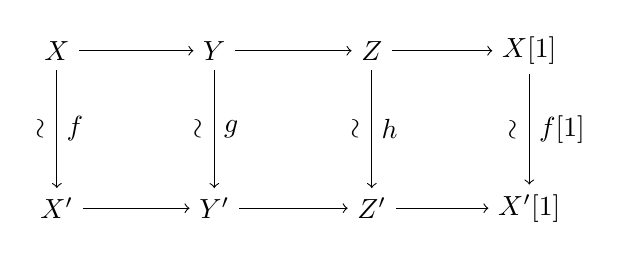
\begin{tikzpicture}

        \node (X) at (-4,2) {$X$};
        \node (Y) at (-2,2) {$Y$};
        \node (Z) at (0,2) {$Z$};
        \node (X1) at (2,2) {$X[1]$};
        \node (X') at (-4,0) {$X^\prime$};
        \node (Y') at (-2,0) {$Y^\prime$};
        \node (Z') at (0,0) {$Z^\prime$};
        \node (X1') at (2,0) {$X^\prime[1]$};
        \draw[->] (X) -- (Y);
        \draw[->] (Y) -- (Z);
        \draw[->] (Z) -- (X1);
        \draw[->] (X') -- (Y');
        \draw[->] (Y') -- (Z');
        \draw[->] (Z') -- (X1');
        \draw[->] (X) -- node[above, rotate=90] {$\sim$} node[right] {$f$} (X');
        \draw[->] (Y) -- node[above, rotate=90] {$\sim$} node[right] {$g$} (Y'); 
        \draw[->] (Z) -- node[above, rotate=90] {$\sim$} node[right] {$h$} (Z');
        \draw[->] (X1) -- node[above, rotate=90] {$\sim$} node[right] {$f[1]$} (X1');
            \end{tikzpicture}
        \end{document}
